\chapter{Modelagem Utilizando Operadores Diferenciais}\label{cap_mod_od}

\thispagestyle{empty}

\markboth{Modelagem Utilizando Operadores Diferenciais}{Operadores de Laplace-Beltrami e Reconstrução de Superfícies Lineares por Partes}

\section{Modelagem geométrica}\label{LB_Int}
\begin{frame}
\frametitle{Resumo do projeto}
\framesubtitle{Introdução}

\begin{figure}[hbt]
	\begin{center}
		\caption{Diagrama de bloco das etapas de desenvolvimento}
		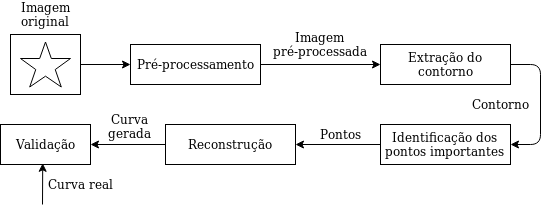
\includegraphics[width=1\textwidth]{img/diagrama.png}
	\end{center}
\end{figure}

\end{frame}


\begin{frame}
	\frametitle{Resumo do projeto}
	\framesubtitle{Exemplo (simples)}
	
	\begin{figure}[ht!]
		\centering
		\begin{subfigure}[b]{0.19\textwidth}
			\centering
			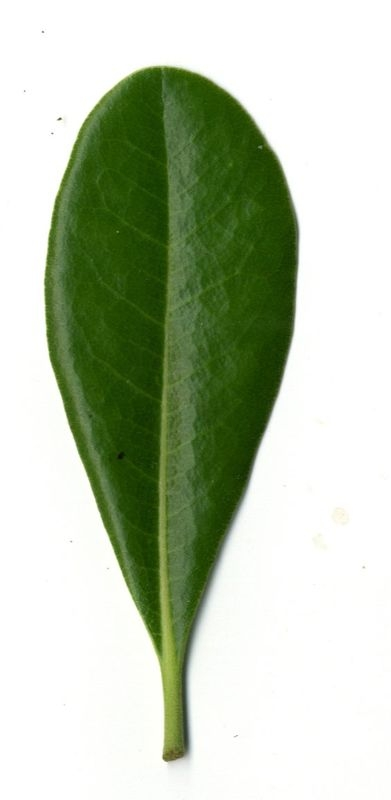
\includegraphics[width=\textwidth]{img/original.jpg}
		\end{subfigure}
		\begin{subfigure}[b]{0.19\textwidth}
			\centering
			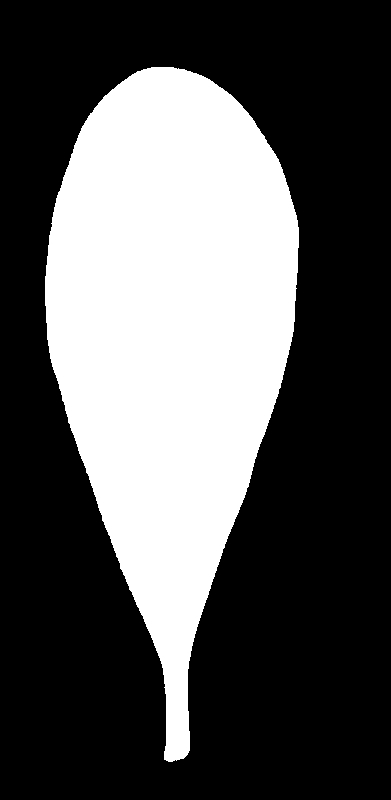
\includegraphics[width=\textwidth]{img/preprocess.jpg}
		\end{subfigure}
		\begin{subfigure}[b]{0.19\textwidth}
			\centering
			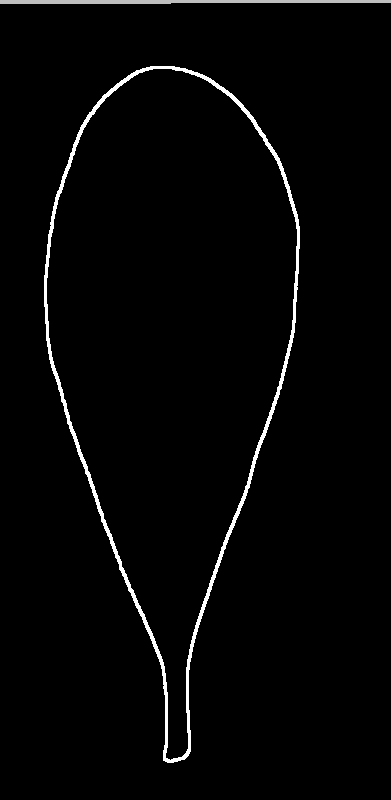
\includegraphics[width=\textwidth]{img/contour.jpg}
		\end{subfigure}
		\begin{subfigure}[b]{0.19\textwidth}
			\centering
			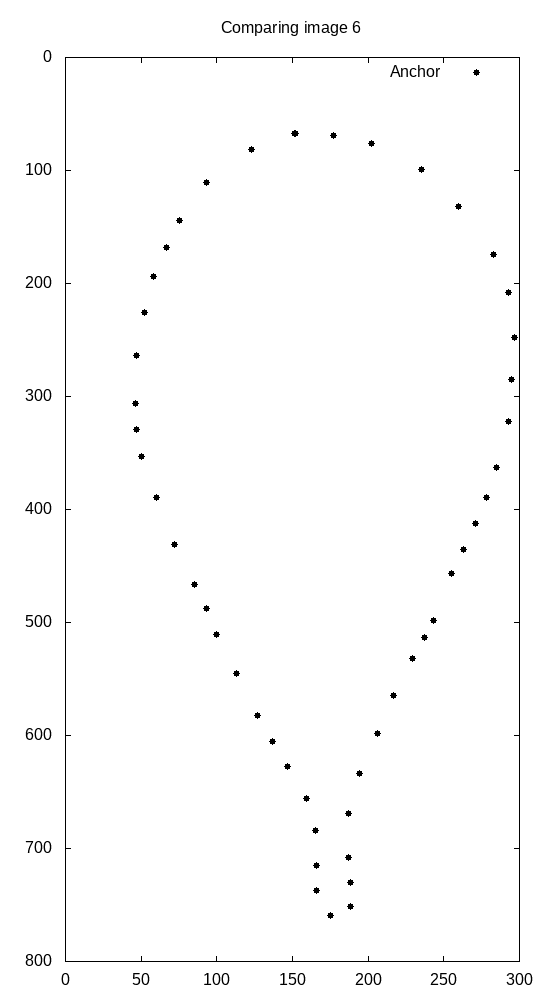
\includegraphics[width=\textwidth]{img/points.png}
		\end{subfigure}
		\begin{subfigure}[b]{0.19\textwidth}
			\centering
			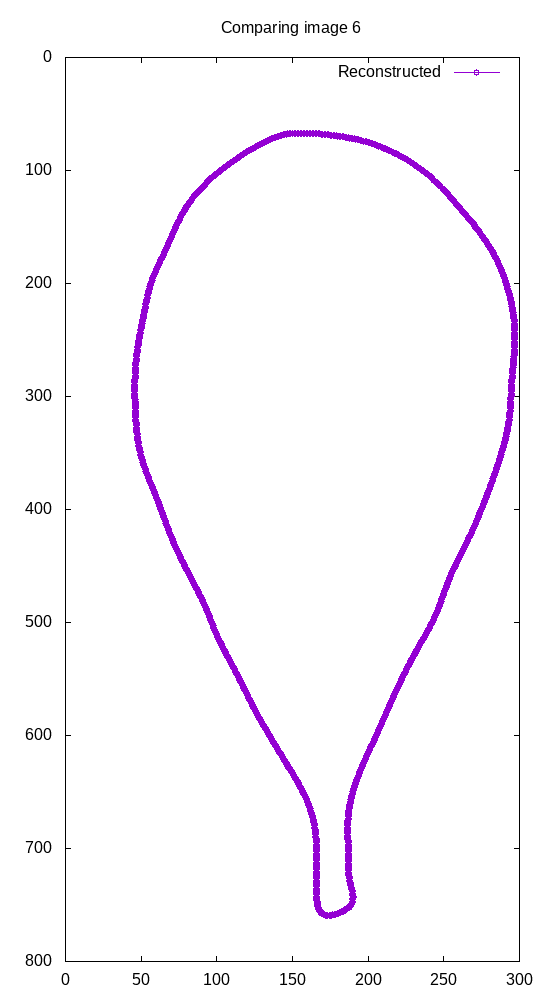
\includegraphics[width=\textwidth]{img/reconstructed.png}
		\end{subfigure}
		\label{fig:editedmesh}
	\end{figure}
	
\end{frame}




\section{Discretização do operador de Laplace-Beltrami}\label{LB_def}
\begin{defi}[Operador de Laplace]
Seja $f$ uma função duplamente derivável de valores reais no espaço euclidiano $\mathbb{R}^n$. O \textbf{operador de Laplace} (também conhecido como Laplaciano), denotado por $\Delta$ ou $\nabla^2$, é definido como o divergente do gradiente:
\begin{equation}
\Delta f = \nabla^2 f = \nabla \cdot (\nabla f) = \text{div} (\text{grad f})
\end{equation}
\end{defi}

A denominação de \textbf{operador de Laplace-Beltrami} vem no contexto de geometria diferencial, em que o Laplaciano pode ser generalizado para operar sobre funções definidas em subvariedades no espaço euclideano e, mais genericamente, em variedades Riemannianas e pseudo-Riemannianas.

\begin{defi}[Coordenadas diferenciais]
	Seja uma malha triangular de $n$ vértices caracterizada por $\mathcal{M} = (V, E, F)$, em que $V, A, F$ são, respectivamente, os conjuntos de seus vértices, arestas e faces. Cada vértice $\mathbf{v}_i \in V$ possui uma representação cartesiana dada por $\mathbf{v}_i = (x_i,y_i,z_i)$. \textbf{Coordenadas diferenciais} (também conhecidas como $\mathbf{\delta}$\textit{-coordenadas}) de $\mathbf{v}_i$ são definidas como a diferença entre a coordenada cartesiana e o centro de massa de seus vizinhos imediatos na malha:
	
	\begin{equation}
	\mathbf{\delta}_i = (\mathbf{\delta}_i^{(x)}, \mathbf{\delta}_i^{(y)}, \mathbf{\delta}_i^{(z)}) = \mathbf{v}_i - \frac{1}{d_i} \sum_{j \in N(i)} \mathbf{v}_j,
	\label{eq_delta}
	\end{equation}
	
	\noindent em que $N(i) = \{j|(i,j) \in E$\} (ou seja, os vértices adjacentes a $i$) e $d_i = |N(i)|$ é o número dos vizinhos imediatos de $i$ (grau de $i$).
\end{defi}

A transformação do vetor de coordenadas cartesianas absolutas ao vetor das $\mathbf{\delta}$-coordenadas, descrita na equação \ref{eq_delta}, também pode ser representada em forma de matriz. Seja $A$ a matriz de adjacências da malha:

\begin{equation}\label{eqMatAdj}
A_{ij} = \begin{cases}
1&(i, j) \in E\\
0&\text{caso contrário.}
\end{cases}
\end{equation}

\noindent e $D$ matriz diagonal tal que $D_{ii} = d_i$ (grau de incidência do nó $i$). Assim, a matriz transformação de coordenadas absolutas para as coordenadas relativas é:

\begin{equation}
L = I - D^{-1}A.
\end{equation}

É mais conveniente utilizar a versão simétrica $L_s$ da matriz $L$, definida por:

\begin{equation}\label{eqMatLaplaciana}
L_s = DL = D - A
\end{equation}

\noindent em que cada célula pode ser calculada da seguinte forma:

\begin{equation}
(L_s)_{ij} = \begin{cases}
d_i&i=j\\
-1&(i, j) \in E\\
0&\text{caso contrário.}
\end{cases}
\end{equation}

A matriz $L_s$ é denominada \textit{Laplaciano topológico} da malha $\mathcal M$. A figura \ref{fig:matrizLaplaciana} ilustra um exemplo de uma simples malha triangular e sua respectiva representação matricial Laplaciana.

\begin{figure}[htb]
	\centering
	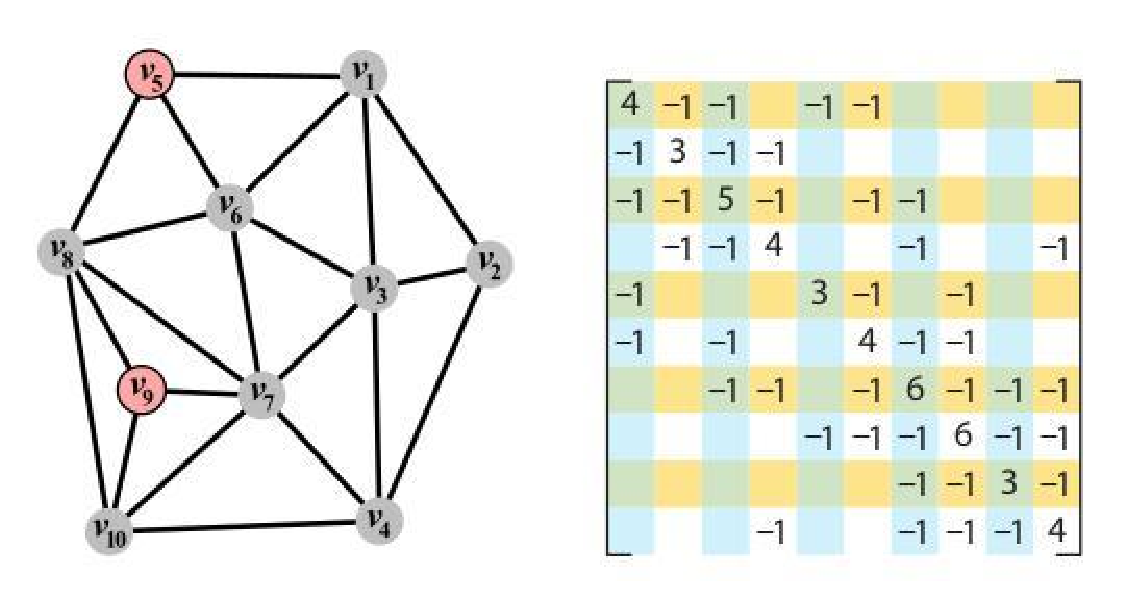
\includegraphics[width=.5\linewidth]{imagens/cap4/meshLaplacian.eps}
	\caption{Uma malha triangular e sua respectiva matriz Laplaciana $L_s$ \cite{sorkine2006}}
	\label{fig:matrizLaplaciana}
\end{figure}

Caso a malha $\mathcal{M}$ seja a aproximação linear por partes de uma superfície suave, as $\mathbf{\delta}$-coordenadas podem ser vistas como a discretização do operador contínuo de Laplace-Beltrami. Pode-se denotar o vetor de coordenadas diferenciais em um vértice $v_i$ como

\begin{equation}
\mathbf{\delta}_i = \frac{1}{d_i} \sum_{j \in N(i)} (\mathbf{v}_i - \mathbf{v}_j)
\end{equation}

\noindent em que este somatório é a discretização da seguinte integral:

\begin{equation}
\frac{1}{|\gamma|} \int_{\mathbf{v} \in \gamma} (\mathbf{v}_i - v) dl(\mathbf{v}))
\end{equation}

\noindent onde $\gamma$ é uma superfície simples e fechada em torno de $\mathbf{v}$ e $|\gamma|$ é o comprimento de $\gamma$. Sabe-se que

\begin{equation}
	\lim_{|\gamma| \rightarrow 0} \frac{1}{|\gamma|} \int_{\mathbf{v} \in \gamma} (\mathbf{v}_i - \mathbf{v}) dl(\mathbf{v}) =  -H(\mathbf{v}_i)\mathbf{n}_i
\end{equation}


\noindent em que $H(\mathbf{v}_i)$ é a curvatura média em $\mathbf{v}_i$ e $\mathbf{n}_i$ é o vetor normal à superfície. Assim, a direção do vetor de coordenadas diferenciais aproxima a direção normal e sua norma aproxima a quantidade proporcional à curvatura média local (o vetor normal escalado pela curvatura média é dito normal da curvatura média). Intuitivamente, isto significa que as $\mathbf{\delta}$-coordenadas encapsulam a forma da superfície local.

Portanto, como ilustra a figura \ref{fig:coordDif}, as coordenadas diferenciais aproximam não apenas as características da forma local da superfície, mas também a direção normal e a curvatura média. 

\begin{figure}[htb]
	\centering
	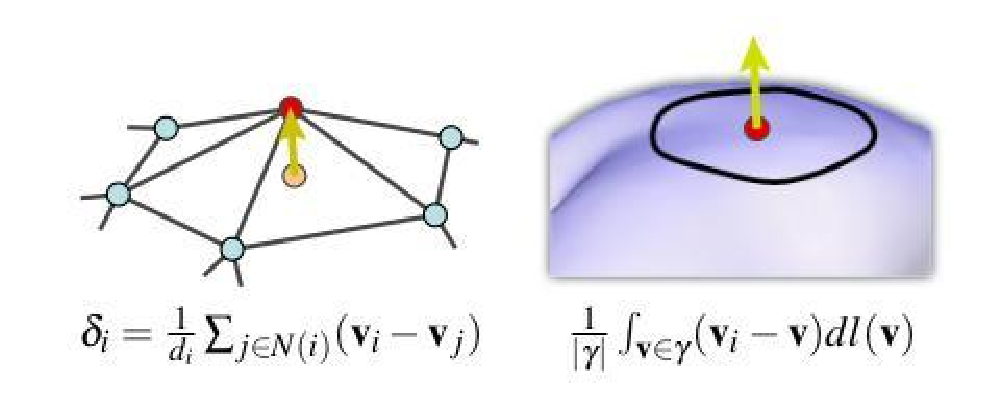
\includegraphics[width=.7\linewidth]{imagens/cap4/difcoord.eps}
	\caption{O vetor da coordenada diferencial em um vértice aproxima a forma local superfície: representação da direção normal e da curvatura média \cite{sorkine2006}}
	\label{fig:coordDif}
\end{figure}

Existem outras formas de se calcular as $\delta$-coordenadas, de forma a se obter melhores qualidades de aproximação. Por exemplo, pode-se ponderar geometricamente o somatório com cotangentes \cite{pinkall:1996}:

\begin{equation}
	\mathbf{\delta}_i^c = \frac{1}{|\Omega|} \sum_{j \in N(i)} \frac{1}{2} (\cot \alpha_{ij} + \cot \beta_{ij})(\mathbf{v}_i - \mathbf{v}_j))
\end{equation}

\noindent em que $|\Omega|$ é o tamanho da célula de Voronoi de $i$ e $\alpha_{ij}, \beta_{ij}$ são os dois ângulos opostos à aresta $(i, j)$. Esta ponderação gera os vetores $\mathbf{\delta}_i^c$, que possuem apenas componentes normais (ao contrário das $\mathbf{\delta}$-coordenadas definidas anteriormente, que podem possuir componentes tangenciais e serem não nulas em 1-anéis planares). Porém, os valores das cotangentes podem ser negativos ou possuírem alguns problemas (em ângulos com valores se aproximando de $\pi$).


%% Juntei as partes de `usos e tecnicas` e `aplicacoes`

\section{Aplicações e exemplos}\label{LB_matlab}
Como dito anteriormente, a representação pelas $\delta$-coordenadas permitem o encapsulamento de informações locais da superfície. Além disso, as matrizes $L, L_s$ e $D$ utilizadas são esparsas, e computacionalmente mais eficientes em questão de memória e tempo de execução.

Com isso, a modelagem utilizando estas coordenadas possuem algumas vantagens interessantes, que serão exploradas nos próximos tópicos.

\subsection{Representação eficiente de formas}

A primeira grande aplicação das coordenadas diferenciais a ser analisada é a representação eficiente de formas, mesmo ao utilizar informações reduzidas do domínio. Se utilizada uma boa base para representação, é necessária apenas uma parcela da função de base para representar toda a geometria \cite{sorkine2004}.

Desta forma, com apenas informações de conectividade da malha e alguns pontos fixados (denominados vértices âncora), é possível aproximar toda a geometria, a partir da resolução do sistema pelo método dos mínimos quadrados:

\begin{equation}\label{eq:sisrecover2}
\left( \frac{L}{\omega I_{m \times m} | 0} \right) \mathbf{x'} = \begin{pmatrix}
0\\
\omega\ c_{1:m}^{(x)}
\end{pmatrix}
\end{equation}

\noindent em que $c = \{v_1, v_2, \dots, v_m\}$ são os pontos âncora escolhidos como amostra, e $\omega > 0$ é o peso de cada restrição (assim como na equação \ref{eq:sisrecover}).

Da mesma forma que anteriormente, de forma gráfica, para facilitar a visualização do sistema:

\begin{center}
	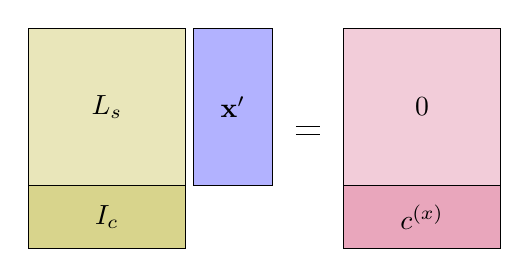
\begin{tikzpicture}
	\filldraw[fill=olive!20!white, draw=black] (0,0) rectangle node{$L_s$} (2,2);
	\filldraw[fill=olive!35!white, draw=black] (0,0) rectangle node{$I_c$} (2,-0.8);
	\filldraw[fill=blue!30!white, draw=black] (2.1,0) rectangle node{$\mathbf{x}'$} (3.1,2);
	\draw (3.4, 0.65) -- (3.7, 0.65);
	\draw (3.4, 0.75) -- (3.7, 0.75);
	\filldraw[fill=purple!20!white, draw=black] (4,0) rectangle node{$0$} (6,2);
	\filldraw[fill=purple!35!white, draw=black] (4,0) rectangle node{$c^{(x)}$} (6,-0.8);
	\end{tikzpicture}
\end{center}

As figuras \ref{fig:ex1rep} e \ref{fig:ex2rep} mostram exemplos de representação de curvas parametrizadas a partir de uma parcela dos pontos originais.

\begin{figure}[htb]
	\centering
	\begin{subfigure}[b]{0.43\textwidth}
		\centering
		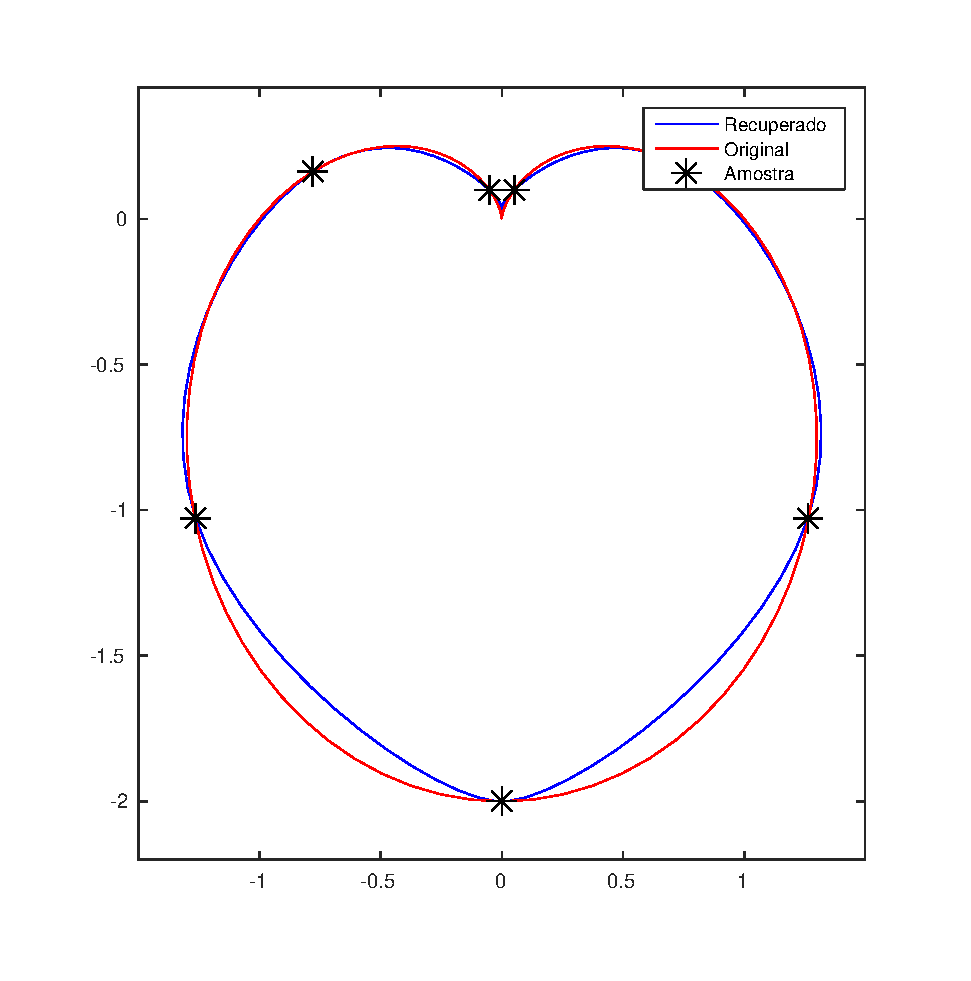
\includegraphics[width=\textwidth]{imagens/cap4/rep_1_8.eps}
		\caption{8 pontos}
		\label{fig:ex11}
	\end{subfigure}
	\hfill
	\begin{subfigure}[b]{0.43\textwidth}
		\centering
		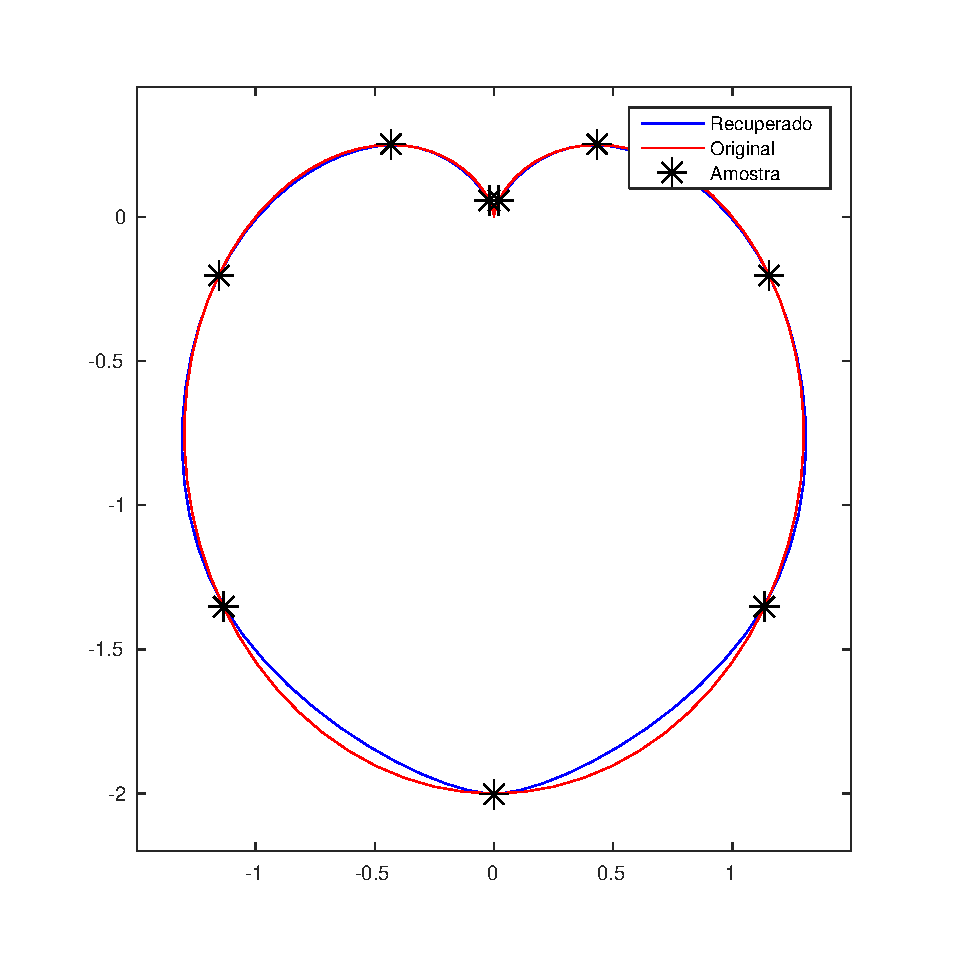
\includegraphics[width=\textwidth]{imagens/cap4/rep_1_10.eps}
		\caption{10 pontos}
		\label{fig:ex14}
	\end{subfigure}
	\hfill
	\begin{subfigure}[b]{0.43\textwidth}
		\centering
		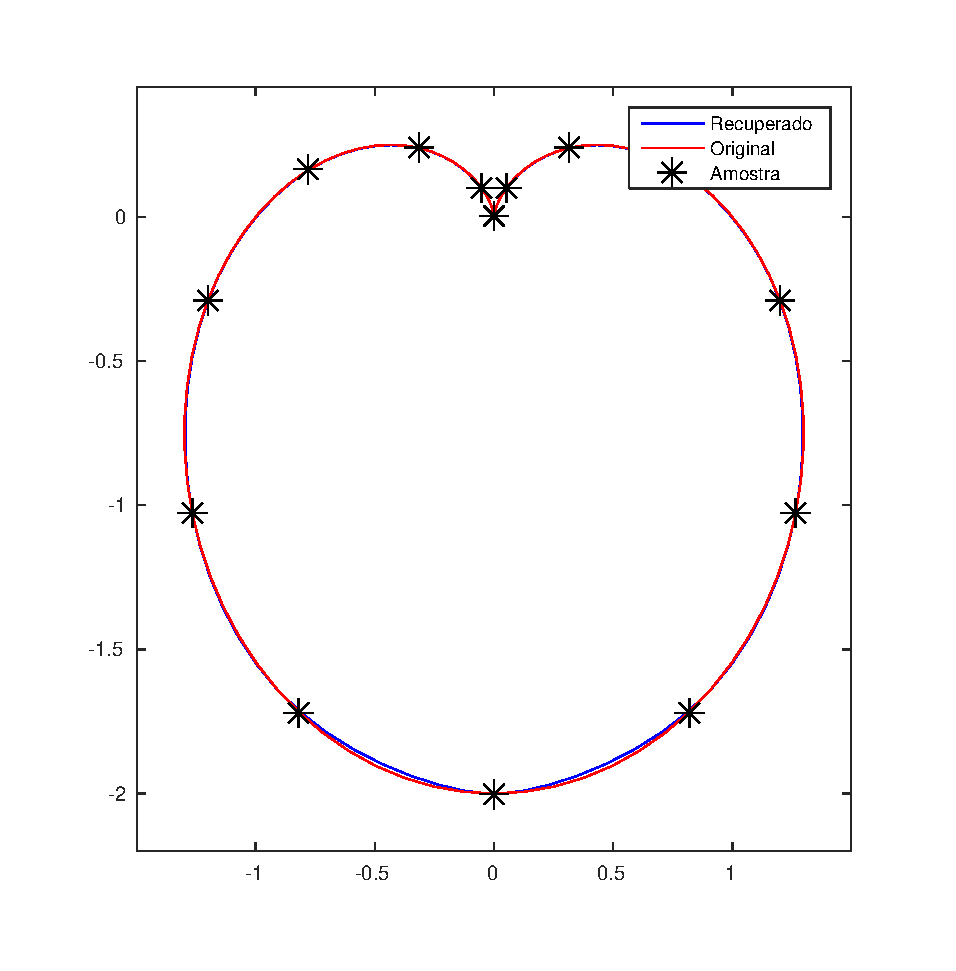
\includegraphics[width=\textwidth]{imagens/cap4/rep_1_15.eps}
		\caption{15 pontos}
		\label{fig:ex12}
	\end{subfigure}
	\hfill
	\begin{subfigure}[b]{0.43\textwidth}
		\centering
		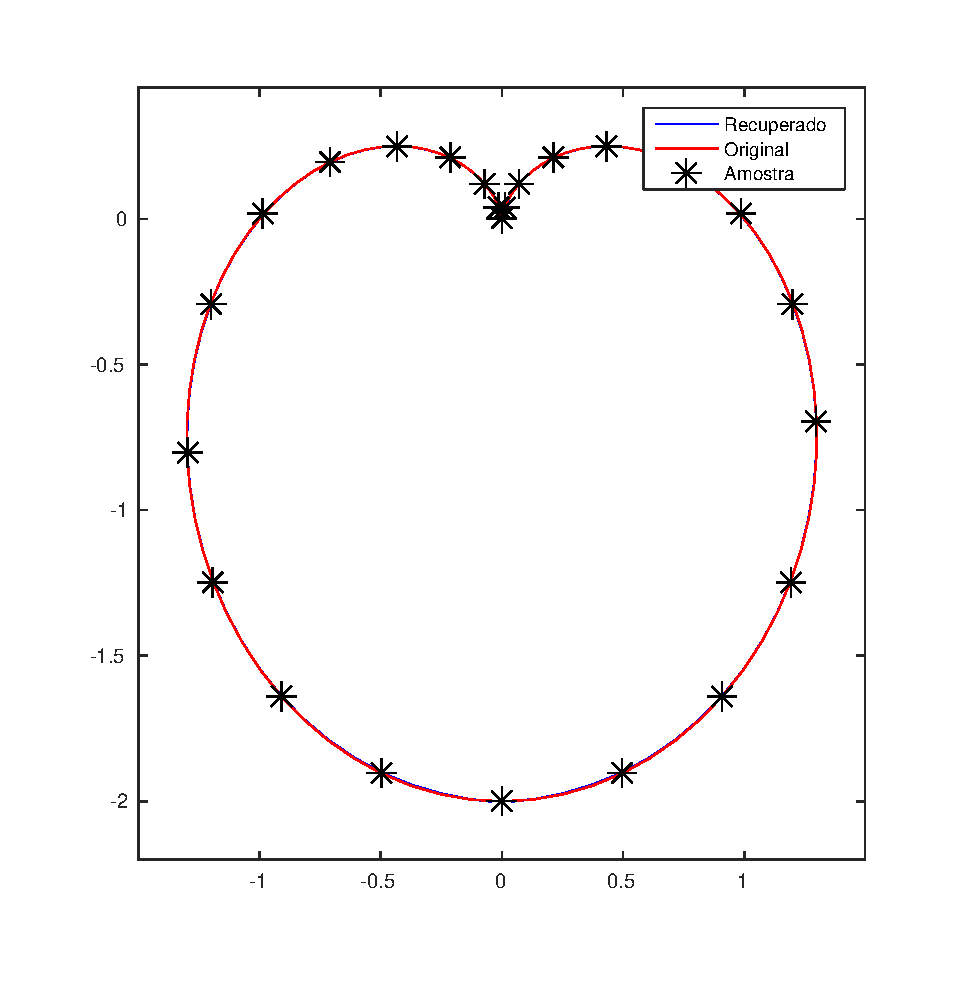
\includegraphics[width=\textwidth]{imagens/cap4/rep_1_25.eps}
		\caption{25 pontos}
		\label{fig:ex13}
	\end{subfigure}
	\caption{Representação da função paramétrica $(x(t), y(t)) = (sin(t) + 0.5 sen(2t), -cos(t) - 0.5 - 0.5 cos(2t))$ utilizando alguns pontos igualmente espaçados como amostra.}
	\label{fig:ex1rep}
\end{figure}


\begin{figure}[htb]
	\centering
	\begin{subfigure}[b]{0.43\textwidth}
		\centering
		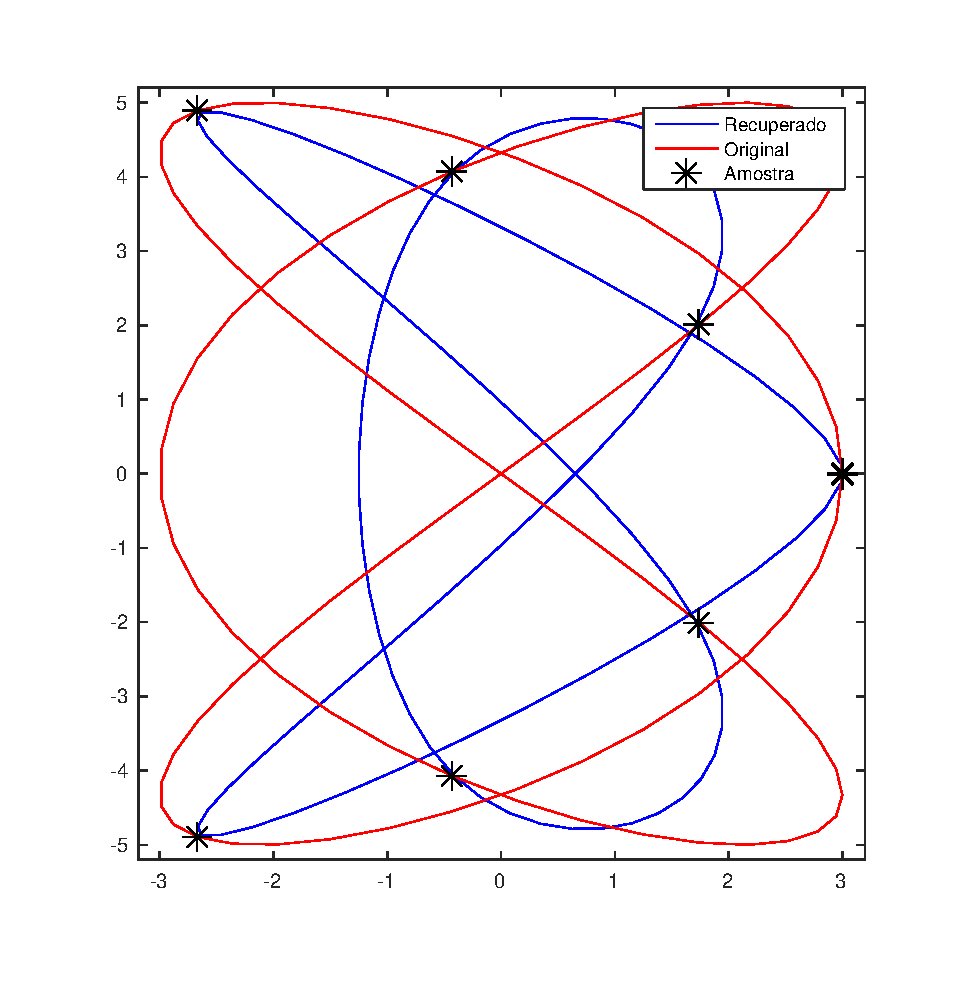
\includegraphics[width=\textwidth]{imagens/cap4/rep_2_8.eps}
		\caption{8 pontos}
		\label{fig:ex21}
	\end{subfigure}
	\hfill
	\begin{subfigure}[b]{0.43\textwidth}
		\centering
		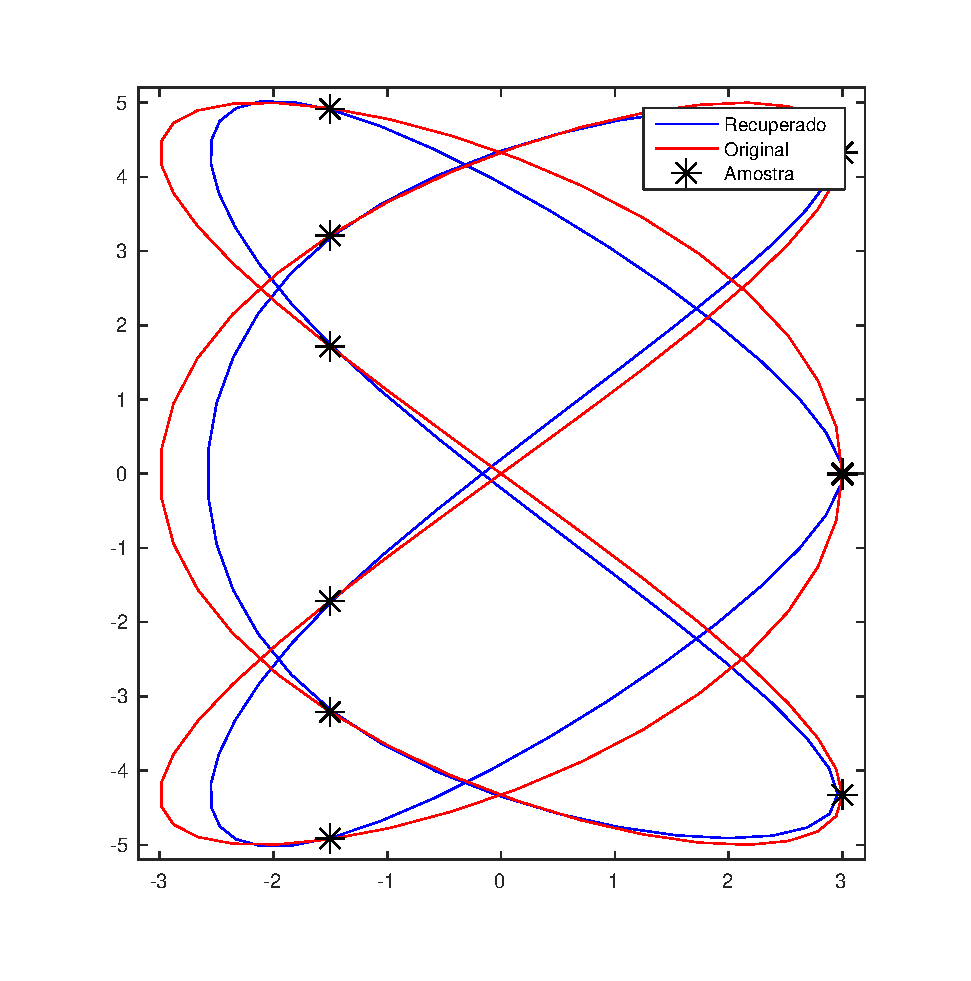
\includegraphics[width=\textwidth]{imagens/cap4/rep_2_10.eps}
		\caption{10 pontos}
		\label{fig:ex24}
	\end{subfigure}
	\hfill
	\begin{subfigure}[b]{0.43\textwidth}
		\centering
		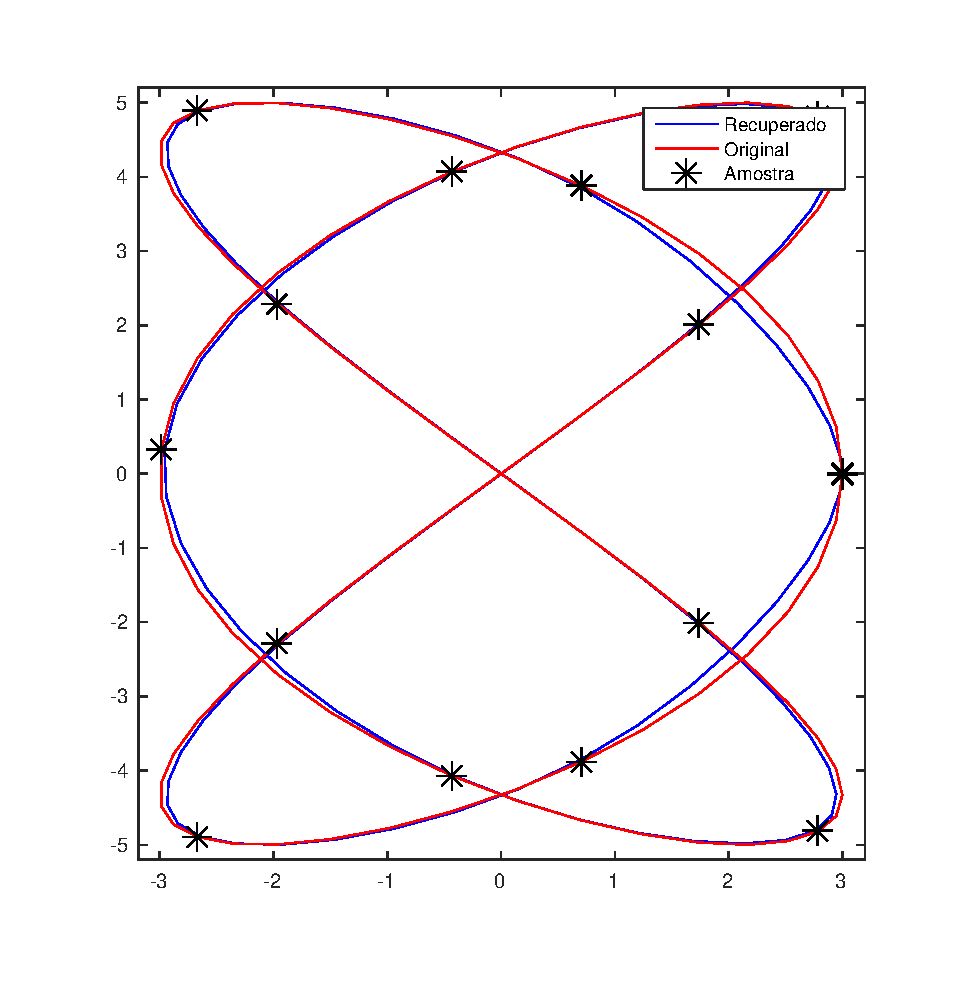
\includegraphics[width=\textwidth]{imagens/cap4/rep_2_15.eps}
		\caption{15 pontos}
		\label{fig:ex22}
	\end{subfigure}
	\hfill
	\begin{subfigure}[b]{0.43\textwidth}
		\centering
		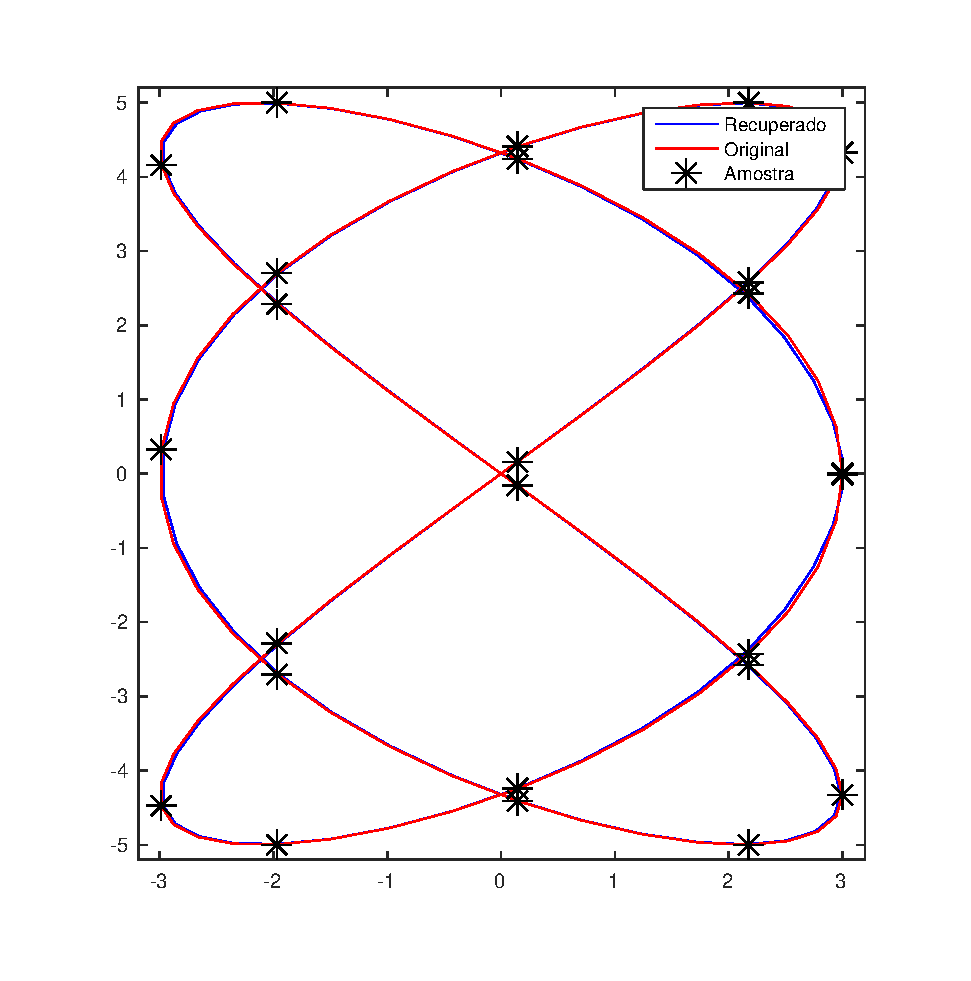
\includegraphics[width=\textwidth]{imagens/cap4/rep_2_25.eps}
		\caption{25 pontos}
		\label{fig:ex23}
	\end{subfigure} %[3 * cos(3 * t); 5 * sin(2 * t)]';
	\caption{Representação da função paramétrica $(x(t), y(t)) = (3 cos(3t), 5sen(2t))$ utilizando alguns pontos igualmente espaçados como amostra.}
	\label{fig:ex2rep}
\end{figure}

Um exemplo de representação de superfícies pode ser visto na figura \ref{fig:ex3rep}, também utilizando alguns pontos igualmente espaçados como amostra (âncora).

\begin{figure}[H]
	\centering
	\begin{subfigure}[b]{0.48\textwidth}
		\centering
		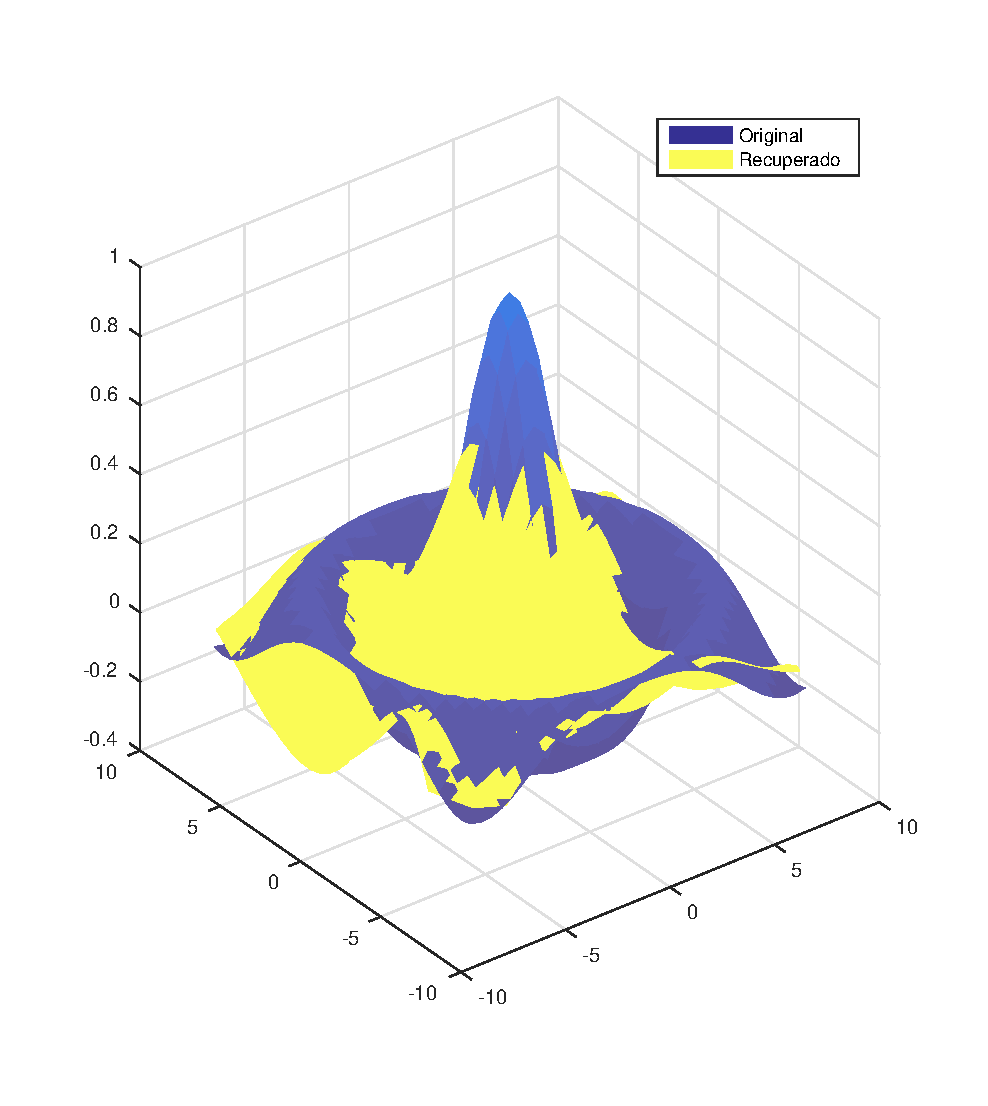
\includegraphics[width=\textwidth]{imagens/cap4/rep3_50.eps}
		\caption{50 pontos}
		\label{fig:ex31}
	\end{subfigure}
	\hfill
	\begin{subfigure}[b]{0.48\textwidth}
		\centering
		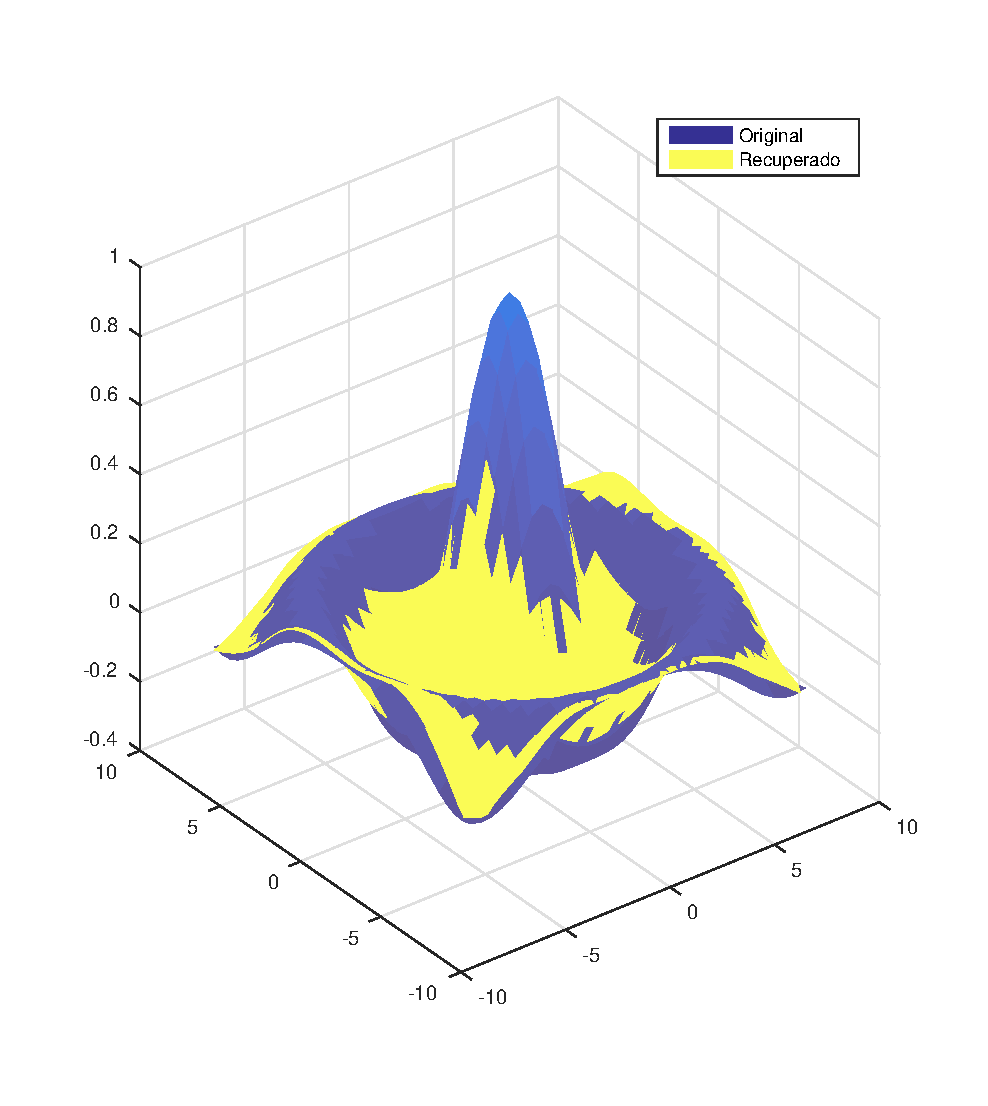
\includegraphics[width=\textwidth]{imagens/cap4/rep3_200.eps}
		\caption{200 pontos}
		\label{fig:ex32}
	\end{subfigure}
	\caption{Representação da função $z(x, y) = \frac{sen (\sqrt{x^2 + y^2})}{\sqrt{x^2 + y^2}}$ utilizando alguns pontos igualmente espaçados como amostra.}
	\label{fig:ex3rep}
\end{figure}

Outro exemplo em espaços tridimensionais pode ser visto na seguinte malha da figura \ref{fig:ex4rep}, utilizando alguns pontos (com índices igualmente espaçados) como âncoras:

\begin{figure}[H]
	\centering
	\begin{subfigure}[b]{0.47\textwidth}
		\centering
		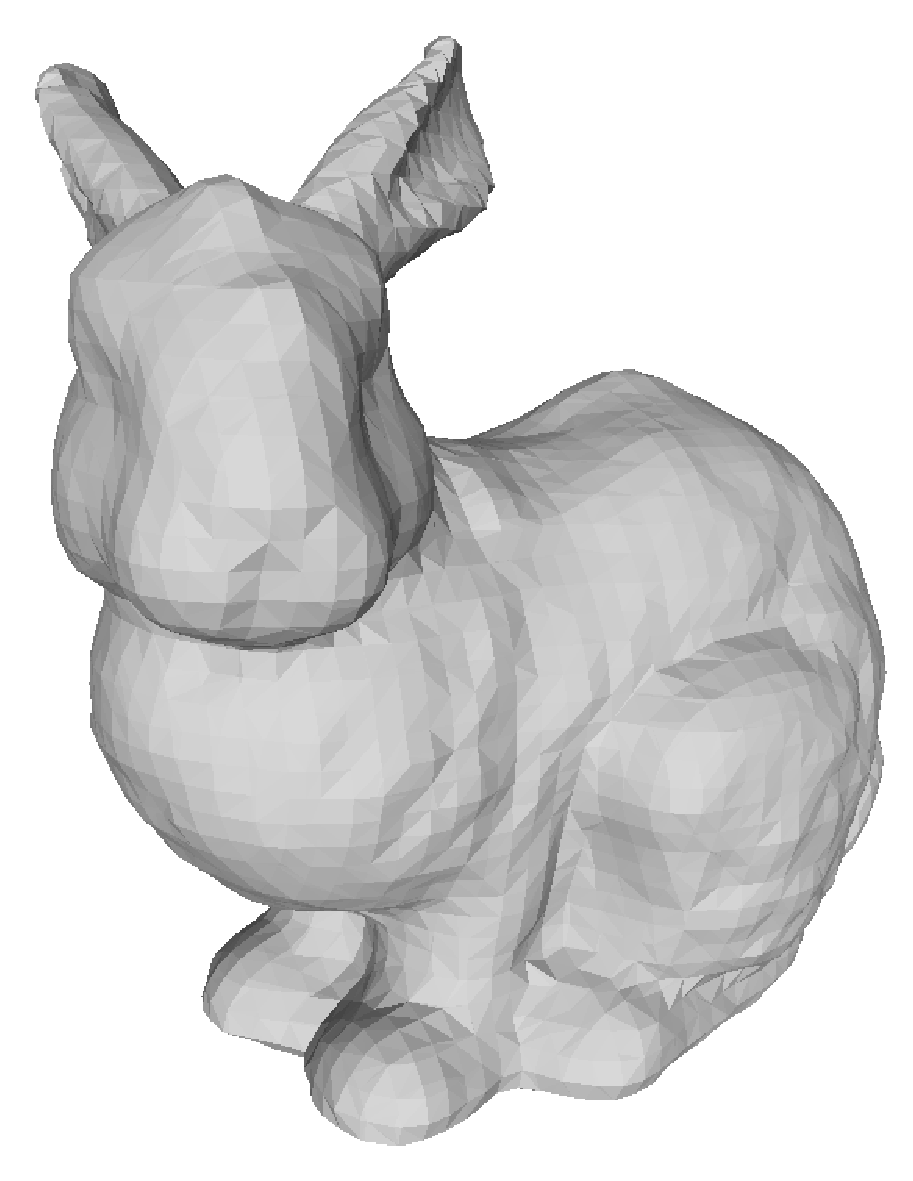
\includegraphics[width=\textwidth]{imagens/cap4/bunny_all.eps}
		\caption{Malha original}
		\label{fig:ex41}
	\end{subfigure}
	\hfill
	\begin{subfigure}[b]{0.47\textwidth}
	\centering
	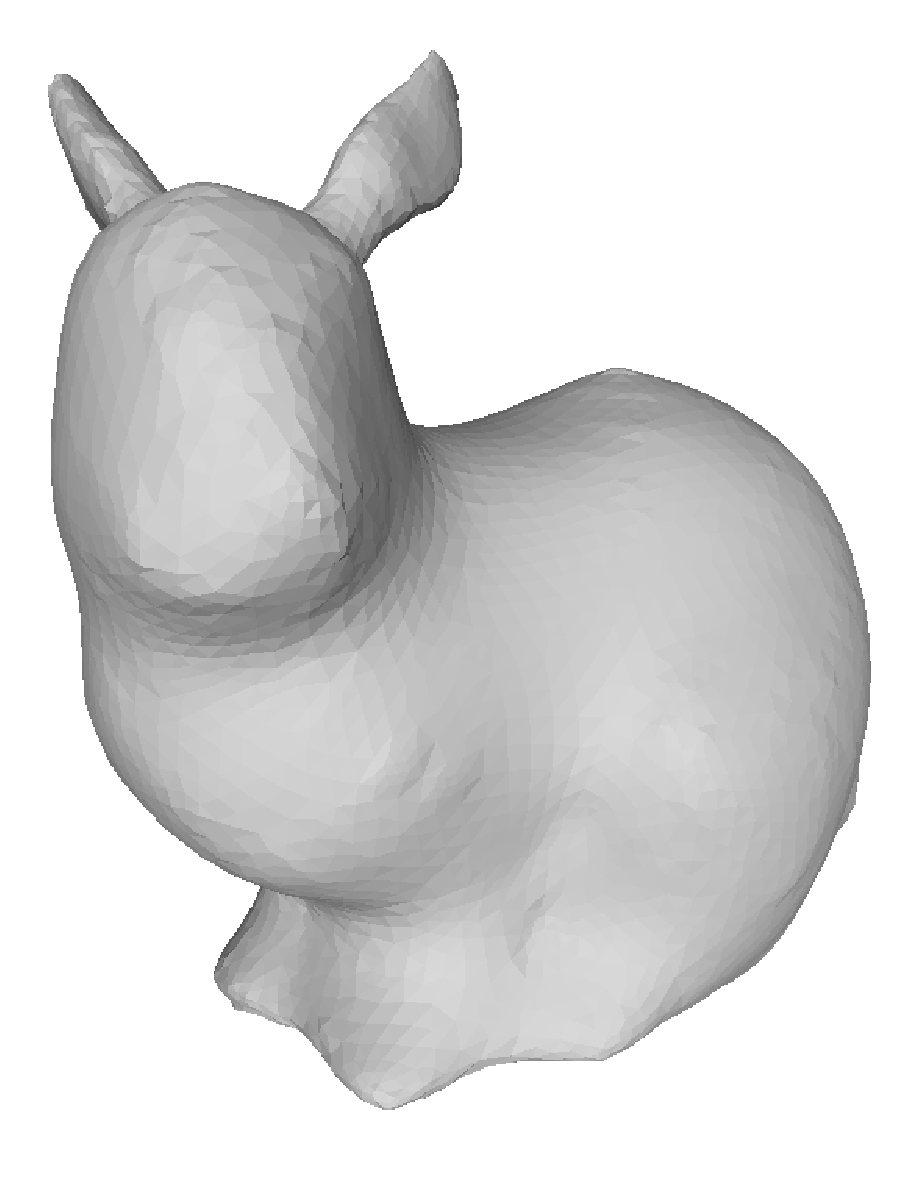
\includegraphics[width=\textwidth]{imagens/cap4/bunny_10.eps}
	\caption{10\% dos pontos}
	\label{fig:ex42}
	\end{subfigure}
	\\
	\begin{subfigure}[b]{0.47\textwidth}
		\centering
		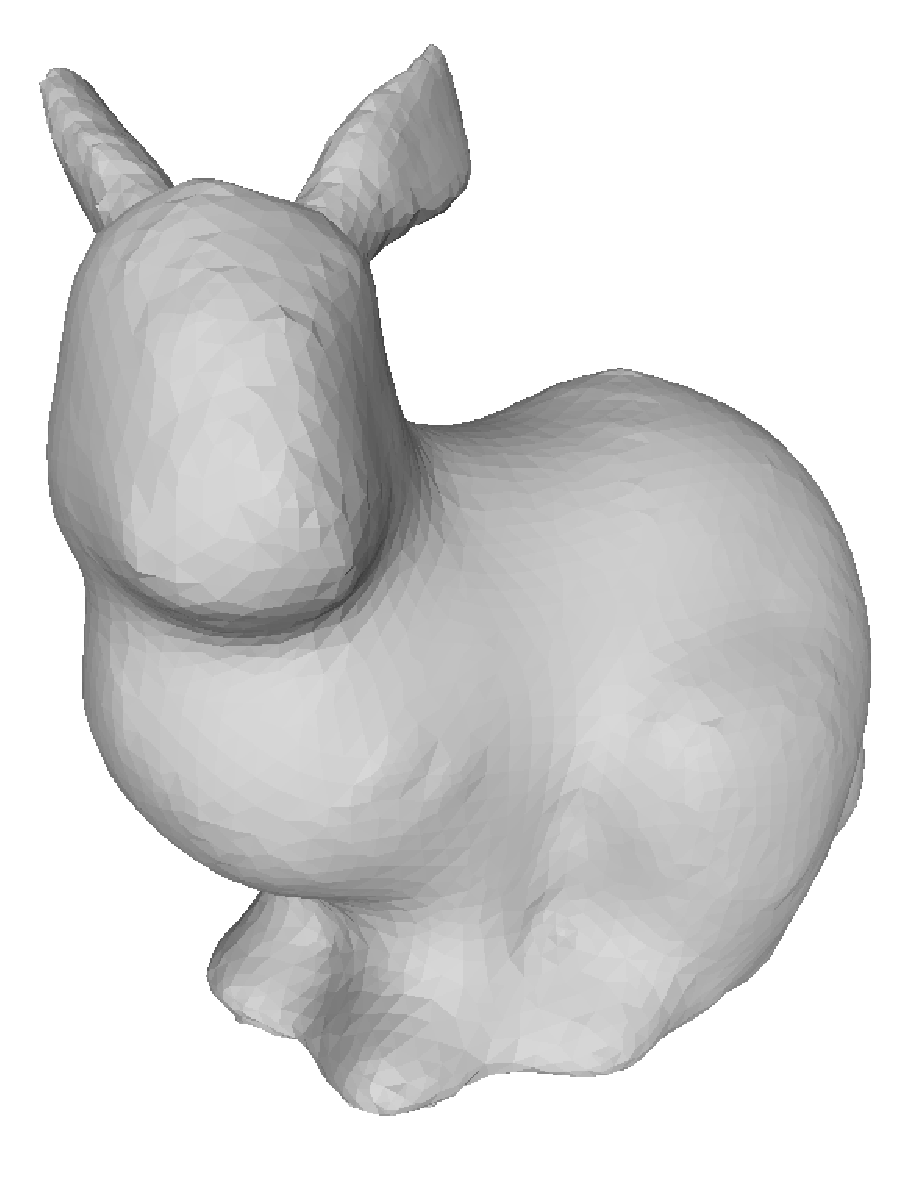
\includegraphics[width=\textwidth]{imagens/cap4/bunny_30.eps}
		\caption{30\% dos pontos}
		\label{fig:ex43}
	\end{subfigure}
	\hfill
	\begin{subfigure}[b]{0.47\textwidth}
		\centering
		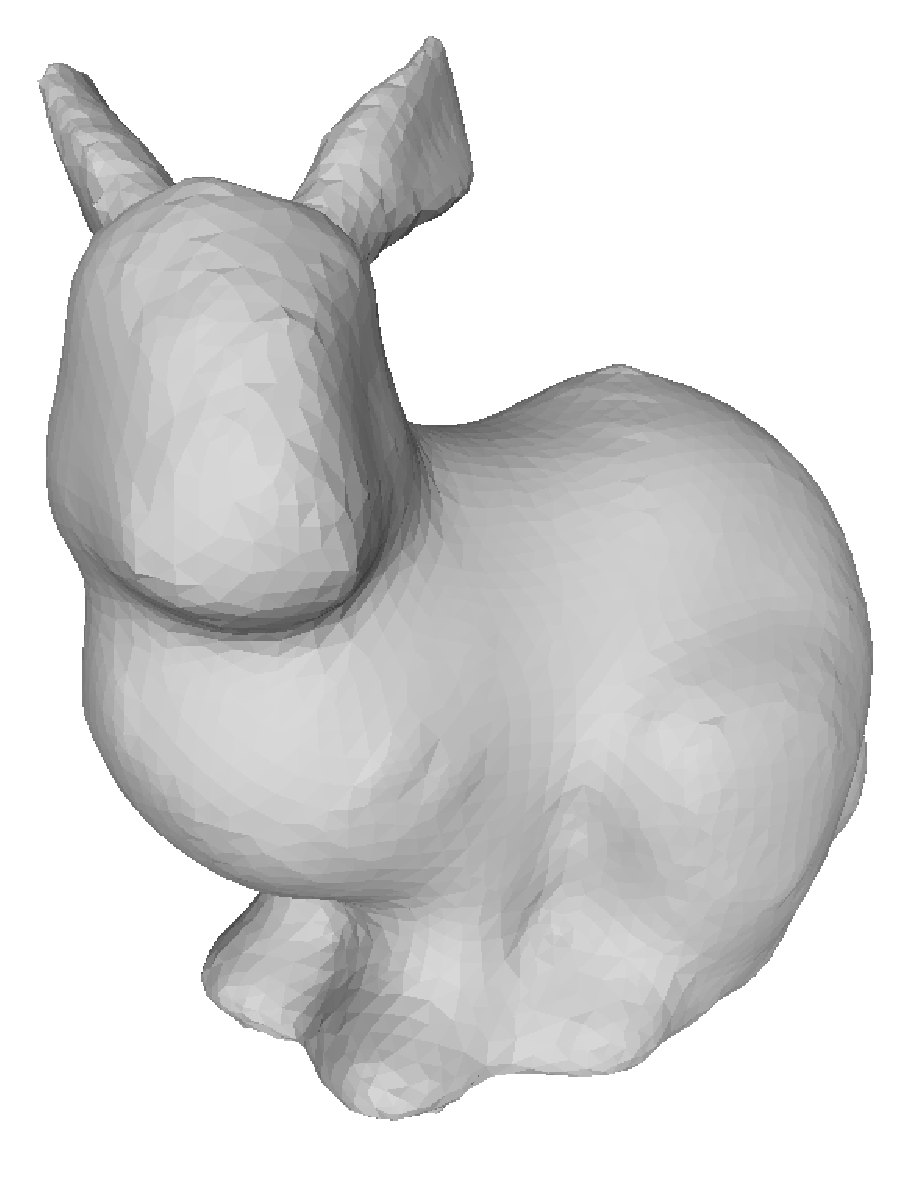
\includegraphics[width=\textwidth]{imagens/cap4/bunny_50.eps}
		\caption{50\% dos pontos}
		\label{fig:ex44}
	\end{subfigure}
	\caption{Representação da malha de um coelho, utilizando apenas uma amostra dos pontos originais como âncoras.}
	\label{fig:ex4rep}
\end{figure}


Nesta figura \ref{fig:ex4rep}, pode-se perceber que alguns detalhes visualmente impactantes do coelho (como o nariz e as pernas) são formados por poucos pontos, e que se estes não forem escolhidos como âncora, os detalhes podem ser perdidos.

\subsection{Edição de malhas}

Outra aplicação interessante das coordenadas diferenciais é a edição de malhas.

Para a edição de alguns vértices da malha, é feito algo similar à reconstrução mostrada anteriormente - porém, além dos pontos âncora, também serão adicionadas restrições dos vértices a serem editados.

Ou seja, além dos $m$ pontos $c = \{v_1, \dots, v_m\}$, são escolhidos $a$ pontos de índices $\{m+1, m+2, \dots, m+a\}$ denominados $e = \{v_{m+1}, v_{m+2}, \dots, v_{m+a}\}$ (novamente, por simplicidade, os pontos são indexados nas primeiras posições, logo após os pontos âncora), e adicionadas as restrições do tipo:

\begin{align}
\mathbf{v}_i &= \mathbf{c}_i, &i \in \{1, \dots, m\}\\
\mathbf{v}_j &= \mathbf{e}_j, &j \in \{m+1, \dots, m+a\}
\end{align}

\noindent e, matricialmente, o sistema pode ser escrito como:

\begin{equation}\label{eq:sisrecoveredi}
\left( \frac{L}{\omega I_{(m+a) \times (m+a)} | 0} \right) \mathbf{x'} = \begin{pmatrix}
\delta^{(x)}\\
\omega\ c_{1:m}^{(x)}\\
\omega\ e_{1:a}^{(x)}
\end{pmatrix}
\end{equation}

Ou seja, De forma gráfica, o sistema a ser resolvido para a edição pode ser visto como:

\begin{center}
	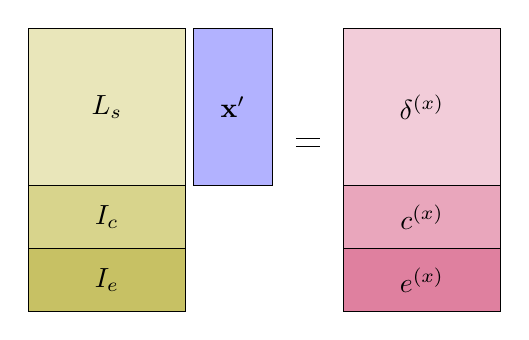
\begin{tikzpicture}
	\filldraw[fill=olive!20!white, draw=black] (0,0) rectangle node{$L_s$} (2,2);
	\filldraw[fill=olive!35!white, draw=black] (0,0) rectangle node{$I_c$} (2,-0.8);
	\filldraw[fill=olive!50!white, draw=black] (0,-0.8) rectangle node{$I_e$} (2,-1.6);
	\filldraw[fill=blue!30!white, draw=black] (2.1,0) rectangle node{$\mathbf{x'}$} (3.1,2);
	\draw (3.4, 0.50) -- (3.7, 0.50);
	\draw (3.4, 0.60) -- (3.7, 0.60);
	\filldraw[fill=purple!20!white, draw=black] (4,0) rectangle node{$\delta^{(x)}$} (6,2);
	\filldraw[fill=purple!35!white, draw=black] (4,0) rectangle node{$c^{(x)}$} (6,-0.8);
	\filldraw[fill=purple!50!white, draw=black] (4,-0.8) rectangle node{$e^{(x)}$} (6,-1.6);
	\end{tikzpicture}
\end{center}

Como é utilizado o método dos mínimos quadrados para a resolução dos sistemas, talvez aconteça alguns erros de precisão. Assim, para minimizar estas falhas, após se encontrar a solução do sistema, pode-se conferir alguns pontos (ou seja, o algoritmo pode, após encontrar os pontos pelo sistema, forçar com que $v'_i = v_i$, para alguns $i$, para que pelo menos estes pontos não sofram erros de precisão).

\begin{figure}[ht!]
	\centering
	\begin{subfigure}[b]{0.45\textwidth}
         \centering
         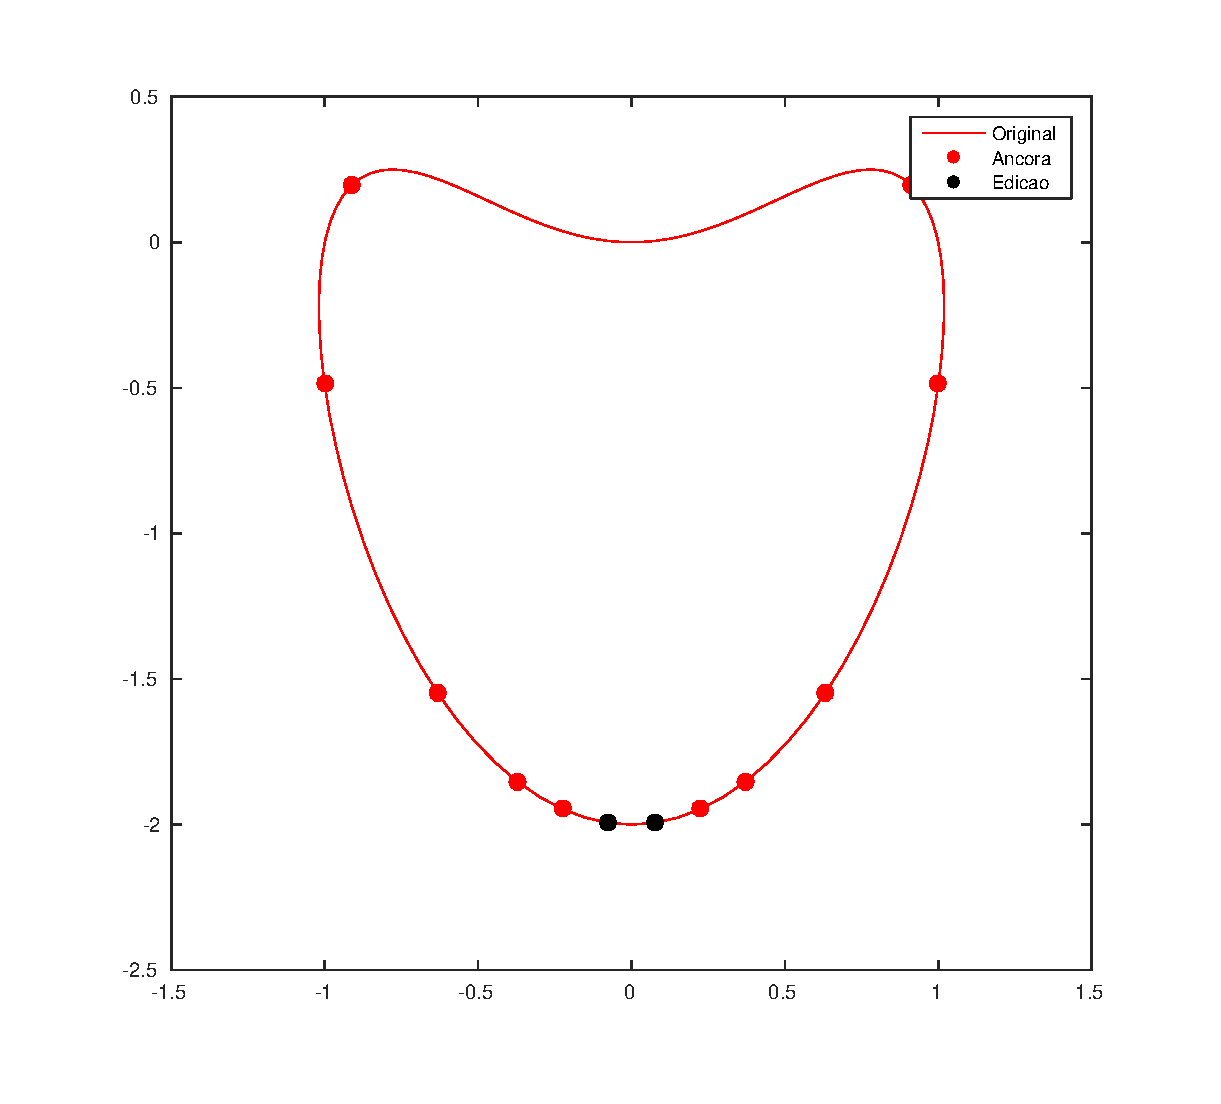
\includegraphics[width=\textwidth]{imagens/cap4/malhaoriginal.eps}
         \caption{Malha original}
         \label{fig:meshorigiedit}
     \end{subfigure}
     \hfill
     \begin{subfigure}[b]{0.45\textwidth}
         \centering
         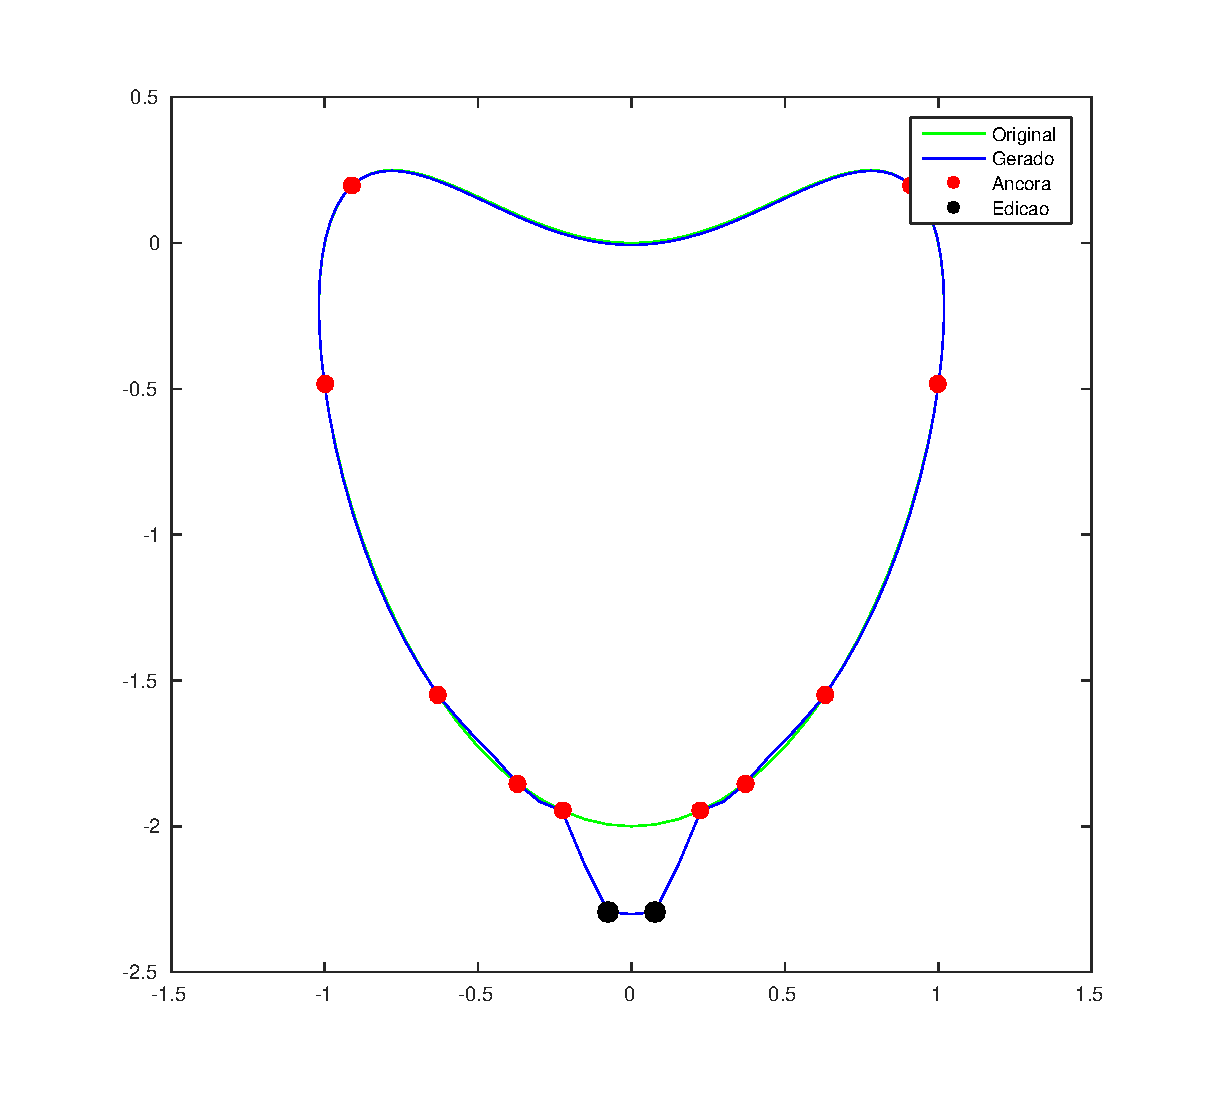
\includegraphics[width=\textwidth]{imagens/cap4/malhaedicao.eps}
         \caption{Malha editada}
         \label{fig:mesheditededit}
     \end{subfigure}
     \caption{Malha antes (\ref{fig:meshorigiedit}) e após edição (\ref{fig:mesheditededit}). Os pontos em vermelho são os pontos de âncora, e os pontos em preto são os editados.}
    \label{fig:editedmesh}
\end{figure}

Este processo pode ser aplicado em malhas tridimensionais, estendendo o sistema de duas $\delta$-coordenadas para três. Ou seja, através da resolução de mais um sistema similar ao exibido acima é possível editar malhas 3D através dos mesmos princípios utilizados para a edição de malhas 2D.  

Além de deformações, também é possível realizar outros tipos de edição, que são discutidas em \cite{sorkine2006}, como inserir marcas d'água, interpolar e suavizar malhas, que não serão discutidos neste livro.



\section{Lista de Exercícios}\label{LB_ListaEx}
\begin{enumerate}
    \item Modelagem geométrica e o uso de malhas poligonais são uma parte intrínseca da computação gráfica. Com uma gama de aplicações e variados usos, a maior parte da humanidade já interagiu com malhas de alguma forma. Sendo assim, quais são alguns destes usos? Procure também encontrar uma malha que você possa manipular de alguma forma. 
    
    \item Construa a matriz de adjacência para uma pirâmide de base quadrada.
    
    \item Construa a matriz de adjacência do exercício anterior em Matlab/Octave.
    
    \item Gere um código em Matlab/Octave que receba uma matriz de adjacências e calcule o laplaciano topológico $L_s$.
    
    \item Gere um código em Matlab/Octave que calcule as $\delta$-coordenadas (com a ponderação padrão vista em \ref{eq_delta}), a partir das coordenadas cartesianas e da matriz de adjacências.
    
    \item Em softwares de visualização de malhas com interação do usuário, é fundamental que o tempo de processamento seja pequeno. Quais as vantagens das matrizes $L$, $L_s$ e $D$ vistas anteriormente em questão de eficiência computacional?
    
    \item Para a representação de formas, é necessário possuir informações de conectividade da malha, como a matriz de adjacências. Como é possível gerar a matriz de adjacência, caso se saiba que a malha é a representação de:
    
\begin{enumerate}
    \item Curva aberta contínua no $\mathbb{R}^2$, em que $v_i \approxeq v(t)$, e os índices estão corretamente ordenados;
    
    \item Curva fechada contínua no $\mathbb{R}^2$, em que $v_i \approxeq v(t)$, e os índices estão corretamente ordenados;
\end{enumerate}

    \item Na seção \ref{LB_matlab}, os pontos âncora foram selecionados como pontos igualmente espaçados. Sugira alguma outra forma para coletá-los, e analise brevemente sua eficiência de representação.

    \item Como visto na seção \ref{Pondera}, alguns dos métodos utilizados para ponderação das $\delta$-coordenadas incluem o uso de pesos cotangentes ou pesos relativos ao número de vizinhos de um vértice. Quais são alguns outros métodos que podem ser utilizados para a ponderação de $\delta$-coordenadas ponderadas?

\end{enumerate}

\subsection{Resoluções}
\begin{enumerate}
    \item De fato, existe um grande número de áreas que utilizam malhas poligonais, desde animação através de computação gráfica, aplicações para decoração de imóveis e arquitetura, modelos computacionais de jogos virtuais, reconhecimento de faces e inúmeras outras aplicações. Também é possível encontrar em diversos repositórios na internet malhas que podem ser carregadas em aplicações que permitem desde a movimentação de câmeras para observação da malha até manipulação direta como torcer, esticar e deformar a malha em geral.
    
    \item Uma possível matriz de adjacência para uma pirâmide em que os pontos 1, 2, 3 e 4 compõe a base é:

$$P = \begin{pmatrix}
0 & 1 & 1 & 0 & 1\\
1 & 0 & 0 & 1 & 1\\
1 & 0 & 0 & 1 & 1\\
0 & 1 & 1 & 0 & 1\\
1 & 1 & 1 & 1 & 0\\
\end{pmatrix}$$

Para transformar essa matriz de adjacência na matriz de uma malha triangular seria necessário adicionar uma aresta entre os pontos 2 e 3 ou 1 e 4.

    \item Vide códigos \textit{geraAdjacenciaPadrao.m} e \textit{geraAdjacenciaPiramide.m}.

    \item Vide código \textit{geraLaplaciano.m}.
    
    \item Vide códigos \textit{geraPesosPadrao.m} e \textit{geraDeltaCoords.m}.

    \item As matrizes descritas são esparsas, o que permite a utilização de algoritmos e estruturas de dados especificas. Além disso, também é possível aplicar algumas decomposições de resolução de sistemas linear (como a decomposição de \textit{Cholesky}) para obter uma maior eficiência.
    
    \item 
    \begin{enumerate}
        \item Caso a malha represente uma curva, e os índices dos nós estejam ordenados conforme o tempo, basta ligar cada vértice $i$ com o predecessor $i-1$ e sucessor $i+1$, para todo $i \in \{2, \dots, n-1\}$. Os extremos (primeiro e último vértices) devem ser tratados a parte: como a curva é aberta, o vértice $1$ está ligado apenas com o $2$, e o vértice $n$ está somente conectado com o $n-1$.
        
        \item Similarmente ao item anterior, basta ligar cada vértice $i$ com o predecessor $i-1$ e sucessor $i+1$, para todo $i \in \{2, \dots, n-1\}$. Porém, como a curva é fechada, além das conexões citadas anteriormente, os vértices $1$ e $n$ também são conectados.
    \end{enumerate}
    
    \item Existem várias sugestões, como pegar os vértices com maior e menor curvatura (podem dar uma melhor representação de curvas), pontos aleatórios (podem ser probabilisticamente melhores ou piores que igualmente espaçados) ou escolher iterativamente os vértices de maneira gulosa (de forma a minimizar a função de erro do método dos mínimos quadrados, que pode ser superior às outras formas discutidas anteriormente).
    
    \item Existem diversas possibilidades para a ponderação de $\delta$-coordenadas. A equação \ref{eq_forpon} descreve a ponderação através dos termos $\mathbf{c_i}$ e $\mathbf{w_{ij}}$, ou seja, alterando estes termos é possível utilizar uma infinidade de métodos de ponderação diferentes. Por exemplo, como mencionado na seção \ref{MD} é possível fazer com que o peso de cada aresta $\mathbf{w_{ij}}$ seja inversamente proporcional ao seu tamanho, isto é, a distância entre $\mathbf{v_i}$ e $\mathbf{v_j}$.
    
\end{enumerate}


%\markboth{Modelagem Utilizando Operadores Diferenciais}{Reconstrução de Superfícies Lineares por Partes}
%\section{Reconstrução de Superfícies Lineares por Partes}\label{proc_recsup}
